\subsection{Deskryptory asymetrii rytmu serca}

Opierając się między innymi na analizie szeregów czasowych $RR$ przy pomocy wykresów \PP{}
grupa badaczy z Katedry i Kliniki Intensywnej Terapii Kadriologicznej i Chorób Wewnętrznych
Uniwersytetu Medycznego im. Karola Marcinkowskiego w Poznaniu oraz Instytutu Fizyki
Uniwersytetu Zielonogórskiego odkryła nowe zjawisko fizjologiczne w zmienności rytmu serca
nazwane asymetrią rytmu serca (ang. - Heart Rate Asymmetry - HRA). Słowo asymetria wyraża interesujące fenomen polegający na
tym, że wkład zwolnień rytmu serca w zmienności krótkoterminowej jest większy niż wkład
przyspieszeń \cite{guasym, biomed, geomasy,  berlinPrzemek,  annals, asym1, asym2,  asym3, asym4, asym5, asym6, asym7, car}, natomiast w zmienności długoterminowej i całkowitej odwrotnie, wkład
przyspieszeń jest większy niż wkład zwolnień \cite{guasym, berlinPrzemek,  annals}.

Elementem geometrycznym względem którego HRA jest definiowana to linia identyczności $l_{I}$ (rysunek \ref{fig:pp_distrib}). Linia identyczności jest jedyną linią posiadającą jasną interpretację fizjologiczną, dzieląca
rytm serca na grupy zwolnień i przyspieszeń.

Opierając się na właściwościach matematycznych wariancji można dokonać podziału wszystkich
parametrów wykresu \PP{}, tzn $SD1^2$, $SD2^2$ i $SDNN^2$, na części dotyczące zwolnień i 
przyspieszeń \cite{geomasy, annals, partitioning}.

\subsubsection{Deskryptory asymetrii krótkoterminowej}
Podział $SD1^2$ dla przyspieszeń i zwolnień wygląda następująco \cite{biomed, geomasy, annals, berlinJa}:
\begin{equation}
SD1^2=\frac{1}{n}\left(\sum_{i=1}^{n_{d}}[r^{\perp\;d}_{i}]^{2}+\sum_{j=1}^{n_{a}}[r^{\perp\;a}_{j}]^{2}\right),\label{SD1_podzial}
\end{equation}
gdzie:
\begin{enumerate}
\item[]$r^{\perp\;d}_{i}$ -- odległość prostopadła przyspieszającego punktu  wykresu \linebreak \PP{} o~indeksie $i$ do linii identyczności,
\item[]$r^{\perp\;a}_{j}$ -- odległość prostopadła zwalniającego punktu wykresu \PP\ o~indeksie $j$ do linii identyczności.
\end{enumerate}
oraz
\begin{enumerate}
\item[]$n_{d}$ -- jest liczbą zwolnień (punktów powyżej linii identyczności),
\item[]$n_{a}$ -- jest liczbą przyspieszeń (punktów poniżej linii identyczności).
\end{enumerate}
Faktycznie występuje jeszcze trzecia grupa punktów leżąca na linii identyczności, a zatem
$n$ będąca całkowitą ilością punktów bedzię zdefiniowana jako:
\begin{equation}
n=n_{d}+n_{a}+n_{on} \label{nki},
\end{equation}
jednakże punkty $n_{on}$ nie wnoszą żadnego wkładu do $SD1$, dlatego można je tutaj pominąć.

Wyrażenie (\ref{SD1_podzial}) składa się dwóch członów które w~naturalny sposób odpowiadają
wkładom zwolnień i~przyspieszeń w całkowitej $SD1^{2}$ 
\begin{equation}
SD1^{2}=SD1_{d}^{2}+SD1_{a}^{2}\label{SD1par},
\end{equation}
gdzie
\begin{equation}
SD1_{d}^{2}=\frac{1}{n}\sum_{i=1}^{n_{d}}[r^{\perp\;d}_{i}]^{2}, \qquad SD1_{a}^{2}=\frac{1}{n}\sum_{i=1}^{n_{a}}[r^{\perp\;a}_{i}]^{2}. \label{STpart}
\end{equation}
Do analizy porównawczej wariancje określone przez wzory (\ref{STpart}) użyte z danymi
pochodzącymi od różnych osób nie są zbyt pomocne, dlatego zostały wprowadzone wielkości
wyrażające znormalizowane wkłady zwolnień i przyspieszeń \cite{geomasy, annals, berlinJa}, tzn.:
\begin{equation}
C1_{d}=\frac{SD1_{d}^{2}}{SD1^{2}}, \qquad C1_{a}=\frac{SD1_{a}^{2}}{SD1^{2}},\label{STnorm}
\end{equation}
przy czym
\begin{equation}
C1_{d}+C1_{a}=1.
\end{equation}

\subsubsection{Deskryptory asymetrii długoterminowej}

Długoterminowa zmienność rytmu serca, $SD2$, obliczana jako wariancja względem linii
centroidu $l_2$ (rysunek \ref{fig:pp_distrib}), w przeciwieństwie do $SD1$, jest
najmniejszym możliwym drugim momentem w tym kierunku \cite{geomasy,annals,berlinJa}. Ponieważ, linia identyczności jest
jedyną linią z jasną interpretacją fizjologiczną to konstrukcja deskryptorów asymetrii dla
$SD2$ jest definiowana względem tej linii, natomiast linia $l_2$ prostopadła do linii
identyczności jest używana tylko do obliczeń.

Podział $SD2^2$ dla przyspieszeń i zwolnień jest koncepcyjnie bardzo podobny do wyrażenia
(\ref{SD1_podzial}), a mianowicie \cite{annals}
\begin{equation}
SD2^2= \frac{1}{n}\sum_{s=1}^{n}r^{||\;2}_{s}=\frac{1}{n}\left(\sum_{i=1}^{n_{d}}[r^{||\;d}_{i}]^{2}+\sum_{j=1}^{n_{a}}[r^{||\;a}_{j}]^{2}+\sum_{k=1}^{n_{on}}[r^{||\;on}_{k}]^{2}\right), \label{LTpart}
\end{equation}
gdzie:  
\begin{enumerate}
\item[]$r^{||}_{s}$ -- odległością punktu \emph{s} od $l_{2}$ wzdłuż linii identyczności,
\item[]$n_{d}$, $n_{a}$ i~$n_{on}$ -- są tak samo definiowane jak dla wzoru (\ref{SD1_podzial}), 
\item[]$r^{||\;d}_{i}$ -- odległość mierzona wzdłuż linii identyczności zwalniającego punktu  wykresu \PP\ o~indeksie $i$ do linii $l_{2}$,
\item[]$r^{||\;a}_{j}$ -- odległość mierzona wzdłuż linii identyczności przyspieszającego punktu  wykresu \PP\ o~indeksie $j$ do linii $l_{2}$.
\end{enumerate}
Podobnie jak w przypadku zmienności krótkoterminej, dwa pierwsze człony we wzorze (\ref{LTpart})
odpowiadają zwolnieniom i przyspieszeniom rytmu serca, jednakże to co odróżnia zmienność
długoterminową to niezaniedbywalny człon zawierający punkty na linii identyczności, czyli:
$1/n\sum_{k=1}^{n_{on}}[r^{||\;on}_{k}]^{2}$ w~(\ref{LTpart}). Wielkość członu związanego
z linią identyczności jest, jeśli tak można wyrazić, zależna sprzętowo, gdyż na ilość 
identycznych (co do wartości) sąsiadujących ze sobą punktów w szeregu $RR$ istotny wpływ ma
precyzja urządzenia pomiarowego. Czym większa precyzja, tym mniej punktów pomiarowych
wpada do tego samego przedziału pomiędzy dwoma dyskretnymi poziomami pomiarowymi, a to
znaczy dążenie do zera liczby punktów na linii identyczności \cite{annals}. 

W pracy \cite{annals} zaproponowano aby człon związany z linią identyczności miał
równy wkład, po połowie, do obu części zwolnień i przyspieszeń, i wielkości tak określone
okazują się bardziej konserwatywne, jak to pokazały testy statystyczne.
 
Podział asymetryczny dla zmienności długoterminowej $SD2$ definiuje się analogicznie jak w 
 (\ref{SD1par}), tzn.:
\begin{equation}
SD2^{2}=SD2_{d}^{2}+SD2_{a}^{2}, \label{SD2part}
\end{equation}
czyli na część pochodzącą od zwolnień i przyspieszeń, a odpowiednie wkłady do wariancji
przy pomocy następujących wyrażeń \cite{annals}:
\begin{eqnarray}
SD2_{d}^{2}&=&\frac{1}{n}\left(\sum_{i=1}^{n_{d}}[r^{||\;d}_{i}]^{2}+\frac{1}{2}\sum_{j=1}^{n_{on}}[r^{||\;on}_{j}]^{2}\right),\label{LTpartdef}\\
SD2_{a}^{2}&=&\frac{1}{n}\left(\sum_{i=1}^{n_{a}}[r^{||\;a}_{i}]^{2}+\frac{1}{2}\sum_{j=1}^{n_{on}}[r^{||\;on}_{j}]^{2}\right). \nonumber
\end{eqnarray}

Uwaga związana ze znormalizowanymi wkładami zwolnień i przyspieszeń przy okazji wzoru (\ref{STnorm})
obowiązuje także dla zmienności długoterminowej, co wyrażają następujące relacje:
\begin{equation}
C2_{d}=\frac{SD2_{d}^{2}}{SD2^{2}}, \qquad C2_{a}=\frac{SD2_{a}^{2}}{SD2^{2}},\label{LTnorm}
\end{equation}
gdzie
\begin{equation}
C2_{d}+C2_{a}=1.
\end{equation}

\subsubsection{Deskryptory asymetrii pełnej}
Opierając się na deskrytorach asymetrii krótko- i długoterminej można dokonać podziału
pełnej zmienności rytmu serca, wzór (\ref{SDNNpartitioning}), na składowe dla zwolnień i
przyspieszeń w następujący sposób \cite{annals}
\begin{eqnarray}
SDNN^{2}&=&\frac{1}{2}\left(\underbrace{(SD1_{d}^{2}+SD1_{a}^{2})}_{SD1^{2}}+\underbrace{(SD2_{d}^{2}+SD2_{a}^{2})}_{SD2^{2}}\right)\\
&=&\frac{1}{2}\left(\underbrace{(SD1_{d}^{2}+SD2_{d}^{2})}_{2SDNN_{d}^{2}}+\underbrace{(SD1_{a}^{2}+SD2_{a}^{2})}_{2 SDNN_{a}^{2}}\right).\nonumber
\end{eqnarray}
lub inaczej jako
\begin{equation}
SDNN^{2}=SDNN_{d}^{2}+SDNN_{a}^{2}, \label{SDNNpart}
\end{equation}
przy czym 
\begin{equation}
SDNN_{d}^2=\frac{1}{2}\left(SD1_{d}^{2}+SD2_{d}^{2}\right),\quad SDNN_{a}^2=\frac{1}{2}\left(SD1_{a}^{2}+SD2_{a}^{2}\right). \label{SDNNpartad}
\end{equation}

Wyrażenie (\ref{SDNNpartad}) w naturalny sposób umożliwia zdefiniowanie	znormalizowanych
wkładów zwolnień i przyspieszeń do pełnej zmienności rytmu serca \cite{annals}
\begin{equation}
C_{d}= \frac{SDNN_{d}^{2}}{SDNN^{2}},\qquad C_{a}= \frac{SDNN_{a}^{2}}{SDNN^{2}}\label{SDNNcontrib}.
\end{equation}
przy czym
\begin{equation}
C_{d}+C_{a}=1.
\end{equation}

Proces konstruowania deskryptorów asymetrii krótko- i długoterminowej jest zobrazowany na
rysunku~\ref{habfig2_2}{.}

Zgodnie z analizą przeprowadzoną w \cite{geomasy,annals} asymetria krótkoterminowa w grupie $N$
badanych osób zachodzi w stopniu istotnym statystyczne, jeśli: 
\begin{equation}
C1_{d}>C1_{a},
\end{equation} 
Natomiast asymetria długoterminowa zachodzi w stopniu istotnym statystycznie \cite{annals}, jeśli:
\begin{equation}
C2_{d}<C2_{a},
\end{equation}
oraz asymetria całkowita jest określona gdy w~grupie $N$ badanych osób, jeśli jest
spełniona poniższej nierówność w stopniu istotny statystycznie \cite{annals}
\begin{equation}
C_{d}<C_{a}.
\end{equation}
Wielkość próby oraz szczegóły metod statystycznych użytych w celu określenia zachodzenia
powyższych warunków zostały podane w pracy \cite{geomasy}.

\subsubsection{Aplikacje kliniczne deskryptorów asymetrii}

Opierając się na danych klinicznych, jak to zostało pokazane w pracach \cite{guasym, biomed, geomasy, annals} 
potwierdzono występowanie asymetrii krótkoterminowej w szeregach odstępów $RR$ u osób 
zdrowych w spoczynku i to w stopniu wysoce istotnie statystycznym. Podobnie, asymetria
długoterminowa została potwierdzona w grupie osób zdrowych w spoczynku w stopniu wysoce
istotnie statystycznym, w pracach \cite{guasym, annals}. Także w tych pracach została potwierdzona
asymetria rytmu serca względem pełnej zmienności rytmu serca, $SDNN^2$, w stopniu wysoce
istotnie statystycznym. Natomiast w pracach \cite{berlinPrzemek, asym1, asym2, asym4, car} można znaleść kliniczne aplikacje
wariancyjnych parametrów asymetrii rytmu serca.

Ponieważ opisane w tym rozdziale deskrytory asymetrii są ze swojej natury pojęciami
całkowicie ogólnymi, mogą być użyte także do badanie asymetrii innych zjawisk medycznych.
I tak, w pracy \cite{hypertension_asym}, została zbadana (i potwierdzona) asymetria krótkoterminowa w zmienności
sygnału ciśnienia tętniczego. Stwierdzono, że jest ona niezależna od HRA.
%\linebreak %przeniesienie związane ze składem
\begin{landscape}
\begin{figure}
\begin{center}
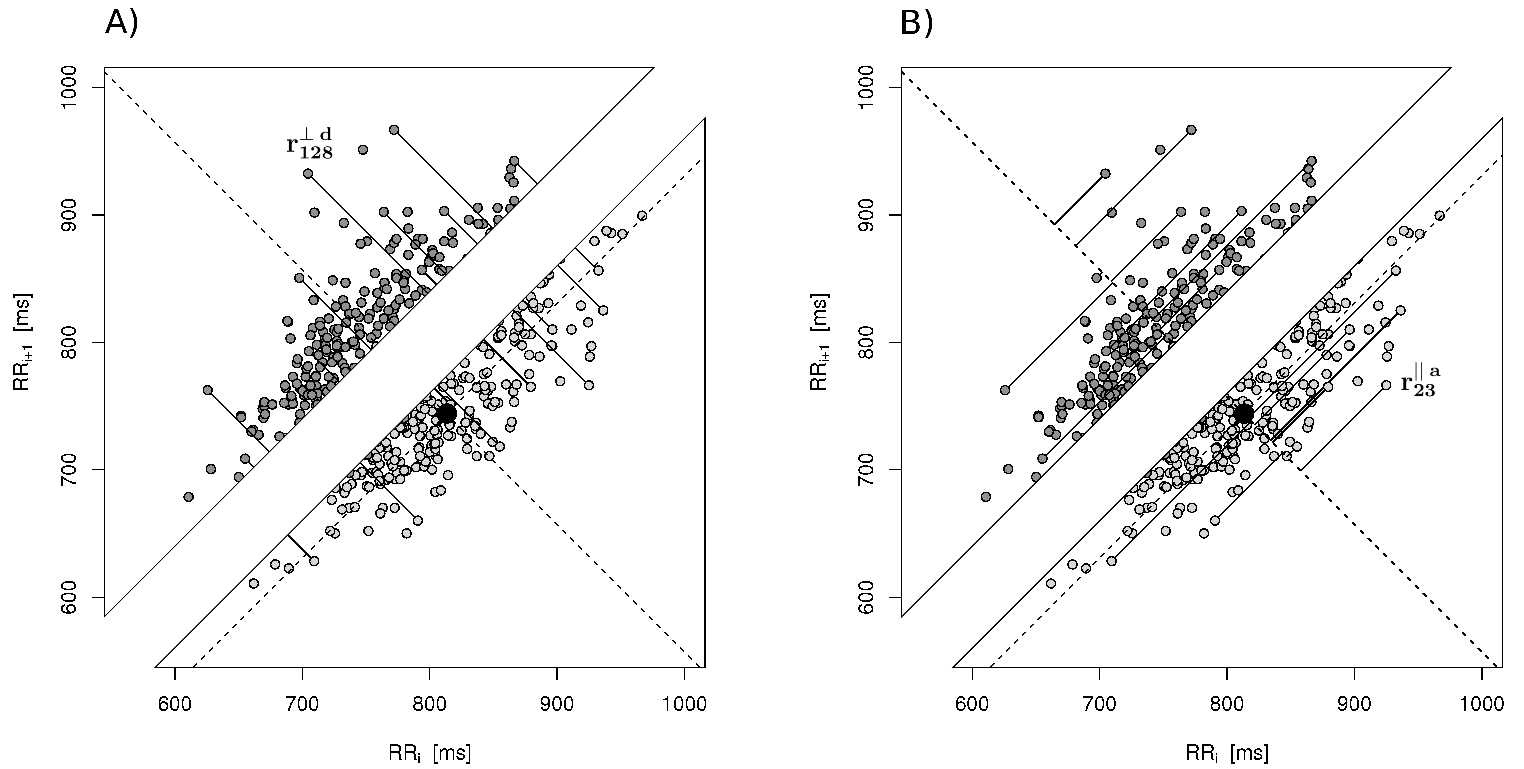
\includegraphics[width=1.5\textwidth]{graph/habfig2_2a}
\caption{W panelu A) przedstawiono konstrukcję deskryptorów krótkoterminowej HRA, a~w~panelu B) proces konstrukcji deskryptorów długoterminowej HRA. Należy zwrócić uwagę, że linia identyczności jest najistotniejszym obiektem geometrycznym w~obu konstrukcjach -- jest ona jedynym kryterium decydującym o~tym, czy dany punkt wnosi wkład do części wariancji ($SD1^2$, $SD2^2$ lub $SDNN^2$) związanej ze zwolnieniami czy przyspieszeniami. $r^{\perp\;d}_{128}$ jest prostopadłą odległością (zwalniającego) punktu wykresu \PP{} numer $128$ do linii identyczności, $r^{||\;a}_{23}$ jest prostopadłą odległością (przyspieszającego) punktu numer $23$ od linii $l_{2}$.\label{habfig2_2}}
\end{center}
\end{figure}
\end{landscape}
\clearpage
